\documentclass[landscape,twocolumn,headrule]{foils}
\usepackage{graphics}
\usepackage{framed}
\usepackage{color}

\begin{document}

\LogoOff %turn off the FoilTeX logo

\MyLogo{
\includegraphics{coklogo_small.png}}

\foilhead{C\"{O}K - Cryptographic One-Time Knocking}

\center{
\includegraphics{coklogo.png}}

David Worth - cesium@hexi-dump.org\\
http://www.hexi-dump.org

\rightfooter{
\includegraphics{bh-us-04-masthead_small.jpg}}

\foilhead{BlackHat Printed Materials}
\LogoOn
\raggedright
\small

These materials were prepared for a more complete exposition on the subject of Cryptographic Port-Knocking, and intentionally do not correspond exactly to the talk (a 20min ``Turbo Talk'') with which they are associated.  Please enjoy the extra content, which is intended to cover background material, some speculative uses for port-knocking in general and C\"{O}K specifically, and a bibliography.

\foilhead{Context and Applications}
In a ``secure`` environment it is optimal to have as few open tcp/udp ports as possible.  In general, a best practice is to block all ports from all hosts, and selectively open the few that are required and appropriate.

However, there are often times when we wish to grant selective access to a set of services to a given host.  This is trivial if the host's IP address is known ahead of time, but if its IP address is dynamic or the host is a public machine (i.e. a kiosk, or public computer lab at a university) then a means of granting and revoking access dynamically is needed.

\foilhead[-.5in]{Define: Port-Knocking}
\center{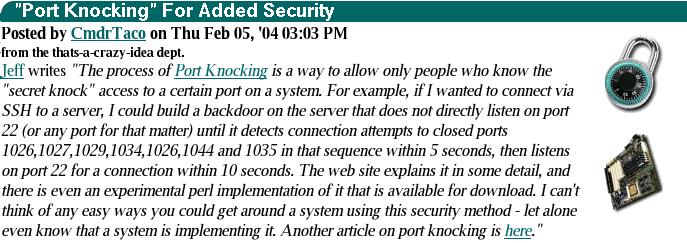
\includegraphics{slashdot_portknocking.png}}

\foilhead{Define: Port-Knocking (con't)}
\raggedright
From \texttt{www.portknocking.org}\cite{portknockingorg}: ``Port knocking is a method of establishing a connection to a networked computer that has no open ports   . Before a connection is established, ports are opened using a port knock sequence, which is a series of connection attempts to closed ports. A remote host generates and sends an authentic knock sequence in order to manipulate the server's firewall''

For the original article on port-knocking see \cite{portknocking-general}.

\foilhead{Port-Knocking is \textcolor{red}{Bogus!}}

Depending on implementation, port-knocking systems are generally susceptible to replay attacks, if not repeated \texttt{nmap(1)} scanning. 

Port-Knocking systems traditionally wait for a shared secret to be passed from an arbitrary host to a ``secure'' host.  This shared secret is nothing more than a (short) sequence of tcp \texttt{connect(2)} calls to a series of ports 

\center{i.e. \texttt{31335,31336,31337 -> Open Sesame, you're \emph{SO} |337!}}

\raggedright
Any host listening in the middle can simply replay the knock if the attacker recognizes that sequence of connections as a knock.

\foilhead[-.5in]{We can \textcolor{red}{\emph{STOP}} Replay Attacks}

By using appropriate cryptographic systems we can prevent replay attacks.  

\emph{One} candidate for such a system is One-Time-Passwords (OTP A.K.A. S/Key).  OTP was designed for insecure transport media (rlogin/telnet actually).  OTP's resilience to replays is based  upon the one-way hash one chooses to use (MD5 or SHA1 traditionally).   See \cite{rfc2289} for the OTP Specifications, \cite{appliedcrypto} for less technical explanations of OTP (pp. 53) and one-way hash functions (ch. 18), or for the more mathematically inclined \cite{handbookappliedcrypto} (ch. 9) has a fairly complete exposition on one-way hash functions.

Detection of attempted replay attacks is also simple: collect valid one-time passwords in a hash, and when you receive an invalid password, check if it is in the hash.  If it is in the hash then someone is attempting to replay the password, and appropriate action can be taken against the attacker (i.e. block them entirely @ the firewall, \texttt{nmap(1)} them, DoS, 0-day, etc...)

\foilhead{Port-Knocking is \textcolor{red}{\emph{STILL} Bogus!}}
If your daemon is insecure you are simply providing a route directly into your firewall!

This is the eternal battle: if you make the code short, and use a good language with proper testing the likelihood of vulnerabilities goes down.  In addition, one can use a ``safer'' language such as Java or LISP in which standard attacks (heap/buffer overflows) are more difficult...

\foilhead{Security is a Process, not a Product}

No product, proprietary/commercial or open-source, is automatically secure, regardless of bragging on the product's webpage.  If we approach the entire process of security more holistically and treat securing a system as a process, viewing security in layers, then port-knocking begins to make sense.

This is the fundamental problem in security to some extent: Can you ever trust your tools?  Can you trust your compiler?  Your OS?  Your hardware?  This is a totally different talk...  but as of now, the answer is \emph{NO!}

\foilhead[-.7in]{But [Product X] automagically solves this...}
There are surely other powerful means of applying an additional layer of security to a system.  Port-Knocking is a lightweight solution whose primary benefits are its flexibility and simplicity.  With higher-level mechanisms one can surely solve the same problems differently, and likely better.

An example of an existing mechanism which attempts to solve a similar problem is OpenBSD's \texttt{authpf} - This is a very cool system with one major drawback, as you are still required to leave OpenSSH bound to \texttt{tcp/22} and accessible from anywhere.  As software goes, OpenSSH does not have a terrible track-record, but it has had its share of problems.  By combining a port-knocking system with \texttt{authpf} one can create a powerful system where no ports need to be open, and authentication is still required!  Regrettably, in a production environment with a great number of users, a great number of knocks are required for this pair to be practical.

To be realistic, the value of port-knocking may not lie in the enterprise security market, but rather a tool for very specific circumstances for use by system administrators and security folks.

\foilhead{Technical Details within Port-Knocking Systems}

In the traditional port-sequence style of port-knocking, the question of turning on and off services at will is trivial.  With a set knock you can open a set of ports, and with a different set knock you can turn off that set of ports.

This is not so easy with One-Time knocks, so one generally must resort to have two sets of knocks, one to open some ports, and another to turn off those ports, and the two sets are correlated.  This is somewhat annoying to say the least...  C\"{O}K tries to solve this

\foilhead[-.7in]{Welcome to C\"{O}K}

\verb;http://www.hexi-dump.org/bytes.html;

Cryptographic One-Time Knocking (C\"{O}K) is a flexible implementation of port-knocking in general,  with a primary goal of supporting cryptographic knock systems (yes, bogus port-sequences are supported just for giggles).

One should note that C\"{O}K, while attempting to be a fairly complete port-knocking solution, should be treated as a proof-of-concept implementation, and should not be used in a production environment.  The concept is valid, and if implemented correctly, should provide the degree of security discussed in this presentation, but there is no guarantee, or even expectation that the implementation discussed lives up to expectations!

\foilhead{One Time Password Systems}

RFC 2289\cite{rfc2289} specifies a the One Time Password protocol, which is based upon the proprietary S/Key authentication system.  The security of One Time Passwords relies on the strength of a one-way hash function (OTP relies on the strength of MD4/MD5/SHA1, though MD4 is deprecated due to technical vulnerabilities).

The system is simple in implementation: a secret pass-phrase and public alphanumeric seed are chosen.  The pass-phrase and seed are concatenated, and hashed iteratively.  The first $N$ iterations are converted into human readable forms (6, 1-4 letter words) and are to be used as passwords.  The $(N\!\!+\!\!1)$ iteration of the hashing routine is stored.  For the first authentication the user sends the $N^{th}$ human readable password, which is in turn hashed and compared to the $(N\!\!+\!\!1)^{th}$ stored hash value.  If they match, the user is authenticated and the $N^{th}$ hash is stored for the next authentication.

\foilhead{One Time Password Systems (con't)}

In OTP / S/Key systems there is a challenge/response protocol:  the challenge consists of a public pass-phrase number and the alphanumeric seed.  These combined with a secret pass-phrase can be converted into a one-time pass-phrase which can be sent in cleartext to a host for login authentication.  This is generally done automatically by a client run locally by the authenticating user.  Another option is to simply record all of the human readable passwords in order, and provide the correct password in response to the challenge.

\foilhead{The C\"{O}K Approach to OTP }

C\"{O}K does away with the challenge/response and replaces the seed with a ``command'' (which is public).  The responsibility of remembering the knock-number is on the user.  The command is simply an alphanumeric string, which is concatenated to the pass-phrase, which in turn specifies the action of the knock.  For instance, a user can have two commands ``lock'' and ``unlock'', which open and close specific ports on their firewall.

The command is concatenated to the pass-phrase when generating the human readable list password lists, and in turn the user has two sets of related passwords, one which opens the firewall, one which closes it, though the two lists may share the same private pass-phrase.  This is analogous the the OTP system of using the same pass-phrase but differing seeds on different machines for simplicity.  The user is then only required to remember one pass-phrase to access various resources.

\foilhead{C\"{O}Kd and C\"{O}KTool}

C\"{O}Kd is the daemon which listens via a JNI wrapper to \texttt{libpcap} for incoming knocks, executes necessary commands, and performs any other maintenance and monitoring for the entire system.  C\"{O}Kd supports robust logging via syslog, and logging directly to a specific file.

C\"{O}KTool is the one-time-knock manager which communicates with C\"{O}Kd via RMI and allows the administrator to create and modify knocks and their associated rules.  To insert, remove, or modify knocks one must use C\"{O}KTool.

\foilhead{Knocking Hello with C\"{O}Knocker}

C\"{O}Knocker is the client which actually passes knocks to the daemon.  The client has the advantage either being run as a java applet on a laptop or other machine, \emph{OR} as an applet in a web-browser, potentially from a non-secure source (though, the security of the applet is then in question...  the applet should probably be hosted by a secure source over SSL with some sort of checksumming.)

To send a one-time knock one simply provides a hostname,  UDP port, and one-time password, and the client wraps it up in a UDP packet and ships it off.  If the knock is accepted by the daemon, the appropriate actions are taken by the daemon.

\foilhead{Usage Scenarios}

\begin{description}
\item[Scenario 1] A user requires access to her WebDAV enabled Apache server on her home machine, but cannot setup SSL for all the domains she hosts for technical reasons.  So she decides on a firewall which blocks all access to the webserver, and enables a knock daemon.
\end{description}

\begin{enumerate}
\item The firewall is up, blocking all access to \texttt{tcp/80}, and the knock server is listening.  Before the user left home, she ran C\"{O}KTool and set up 2 knocks, sharing a pass-phrase but with differing commands.  Each knock has 100 human readable passwords calculated, though she intends on accessing the server from her laptop, so she does not record the passwords, she merely remembers her pass-phrase, the command names, target port number, and the number of knocks in each knock, in this case 100.

\foilhead[-.5in]{Usage Scenarios (con't)}

\item The user is at an internet caf\'{e}, and wants to update her calendar in iCal, which is stored on her WebDAV enabled server at home, so she runs C\"{O}Knocker on her local machine.  Since she has never logged in before, she knows that her knock number is 100.  In C\"{O}Knocker she inputs her pass-phrase, command name, knock number, and target port, and calculates the human readable password.  She then sends the knock.
\item C\"{O}Kd receives the knock, validates it, and executes its stored commands; in this case \texttt{tcp/80} is opened to her source IP.
\item The user then uses iCal and updates her calendar, verifying that she is, in fact, late for her important meeting with a client.
\item The user then changes the command in C\"{O}Knocker, re-calculates the pass-phrase, and sends the knock.  Since all of the other information is the same based on her knock generation, no other changes are necessary.  (Though information is not stored over restarts of the applet)
\item C\"{O}Kd repeats the above steps, this time closing \texttt{tcp/80} to her source IP.
\end{enumerate}

\foilhead[-.7in]{Usage Scenarios (con't)}

\begin{description}
\item[Scenario 2] The above user is leaving on vacation to SE Asia, and does not want the trouble of carrying along her laptop and keeping track of it to prevent theft.  Regrettably, since the user is fairly aware of security happenings, she is aware of a 0-day in her secure shell daemon, for which there is no immediate patch, so she blocks all connections to \texttt{tcp/22}  at her firewall.
\end{description}

\begin{enumerate}
\item As in \textbf{Scenario 1} the firewall is up, the knock daemon is running, and there are two registered knocks, one for opening \texttt{tcp/22}, and one for closing it.  The major difference is that the user is bringing no tech-toys on her vacation, so she writes down her pass-phrases on a piece of paper in her wallet.  The user also uploads the C\"{O}Knocker applet, along with a trusted secure shell applet, to a public website running over SSL, which will be accessible from an internet caf\'{e} or kiosk during her vacation.  As an added precaution, and just out of curiosity, the user also adds a set of replay attack rules, which log replay attacks, and then portscans the attacking host.

\foilhead[-.5in]{Usage Scenarios (con't)}

\item Once on vacation, the user decides to check her e-mail from a kiosk.  She accesses the public website, and launches the C\"{O}Knocker applet, submits the proper information along with the first knock on her list.
\item C\"{O}Kd validates her knock and opens \texttt{tcp/22}, and the user checks her email via her secure shell applet.
\item The user then closes the port via the client applet again, and goes about her business.
\item Unbeknownst to the user, the kiosk's owner tracks all traffic from the kiosk, and notes the odd traffic from the port knocker.  He then portscans the secure host, and sees that \texttt{tcp/22} is closed, and guesses that the strange packets, followed by a secure shell session, followed by similar strange packets are a port-knocking system, and attempts a replay attack.
\item Almost immediately after the replay attack attempt, after the attacker has given up because no ports opened after the replay, the attacker's IDS notes that it has been portscanned by the target of his replay attack...
\end{enumerate}

\foilhead{Managing knocks is \textcolor{red}{\emph{Painful!}}}

There are a number of solutions to this problem:
\begin{itemize}
\item The Russian Space Program Way: pencil and paper; yes, it is fairly pedestrian, but it will work reliably and without crashes (though it is susceptible to clothes-washing!).
\item Save the text-file full of one-time passwords to your PDA, and delete them as you use them.
\item Write a more sophisticated client for your PDA to do the above in an automatic and secure way which keeps the list encrypted in storage.
\item C\"{O}Knocker only requires that you remember the knock number, passphrase, and command one wishes to use, and handles the rest, including the calculation of human readable passwords
\end{itemize}

\foilhead[-.5in]{Alternative uses for C\"{O}K}

Thus far, the only use for port-knocking which has been discussed in public is opening specific ports on a firewall, but this is fairly limited.

Other Potential Uses:
\begin{itemize}
\item An authenticated in-band limited messaging protocol.
\item Verifiable IP address tracking during a penetration test for purposes of documentation.  This may be handy during a penetration test to record the IP addresses of compromised hosts... (maybe)
\item Verification of remote code execution:  Shellcode which uses \texttt{send(2)} to send a one-time knock to a server, from which it then receives its full payload to deploy, should be simple to write .  This allows for a form of authenticated syscall-proxying, or uploading of machine specific tools (rootkits, etc...)
\end{itemize}

\foilhead{Steganography and Port-Knocking}

It is rather odd to see UDP packets flying around the net with 6 whitespace separated ``words'' in them, without any context, especially on everyone's favorite port: 31337.

One can easily write a new knock extending the \verb;UDP_OTP_Knock; class (residing in the \texttt{cokd} package) to only listen for knocks on \texttt{udp/53} which look like legit DNS lookup requests with ``funny-looking'' addresses.  One can then write a new client which wraps the knock in an appropriate DNS lookup packet, and the client will ignore the response from the DNS server (if one is running, and one should be for maximum effectiveness).  This is particularly effective on a DNS server as it will not likely be noticed, except by the random log message regarding failed DNS lookups.  

\foilhead{Steganography and Port-Knocking (con't)}

Taking this one step further, one could simply write a daemon which binds \texttt{udp/53} and acts like a DNS server (on a non-DNS serving machine), and rather than requiring all of the overhead of C\"{O}Knocker, one could simply knock using your favorite DNS tool (i.e. \texttt{nslookup}, \texttt{dig}, etc...)

Knocking by standard browser without an applet is also a possibility.  One could hack a knock to watch for DNS requests stemming from standard web requests.  For example, if one owns (or ownz0rs) the \verb;knockable.org; domain, then a knock could be performed by surfing to \verb;http://[OTP].knockable.org;  The domain lookup will fail, but the knock listener may still respond as it is listening passively!

\foilhead{Out-of-Band Knocking}

SMS is not only super-addictive and popular, but it has potential for use in One-Time knocking systems.  It is conceivable to use a cheap local-access-only cellular phone (i.e. Cricket, etc...) with SMS enabled and an over-the-counter USB / serial cable combined with a system driver for the phone to transmit a given knock.  Even better, with the modern generation of high-end phones, a custom OTK client can be written to handle this.

This allows one to bypass the ``usual'' networking hardware, which may or may not be controlled by ``the bad guys''.  Surely the SMS network can be controlled by those same bad guys, but it is another layer of difficulty for an attacker.

\foilhead{Technical Issues with C\"{O}K}

Since C\"{O}Kd uses a \texttt{libpcap} wrapper, it does no stream reassembly, so if the knock packets are fragmented the knocks will not succeed...  Maybe some basic stream reassembly is appropriate for the next version.

\foilhead[-.5in]{Man-in-the-Middle Attacks against C\"{O}K}

If an attacker completely controls traffic between a knocking host and a target machine then there is (at least) one potential attack against the system.

\begin{description}
\item[Scenario:]  An attacker may record and drop a given knock en-route to a target host.  The attacker then sends the knock herself, and mounts an attack on the now open services.  The legitimate user cannot connect to the services.  A reasonable assumption on the part of the user is that the wrong number knock was sent, and sends the next knock in the sequence.  At this point the attacker has two options:  a) Pass the second knock, allowing the user to assume they missed a knock and move on.  This is \emph{great} as the ports will \emph{never} be locked down as the attacker will never send the shutdown knock by choice.  b) Collect the second knock, and repeat above scenario.
\end{description}

\foilhead{Thank You}

Thank you to Jim Prewett (download@hpc.unm.edu) for his encouragement with C\"{O}K, his forcing me to submit my BlackHat CFP, and for this proofreading of these slides.

Thank you to Dino Dai Zovi for his early encouragement regarding the principals of OTP combined with Portknocking.

Thank you to Meghan Holmes for her encouragement, assistance, and understanding during the stressful hours of preparing this presentation.

\foilhead[-.7in]{Bibliography and Links}
\tiny
\begin{thebibliography}{99}
\bibitem{portknocking-general} Krzywinski, M.  2003.  ``Port Knocking: Network Authentication Across Closed Ports.'' SysAdmin Magazine 12: 12-17.
\bibitem{portknockingorg} \texttt{www.portknocking.org} - \verb;http://www.portknocking.org;
\bibitem{handbookappliedcrypto} Menezes, Alfred J, et al. \underline{Handbook of Applied Cryptography} - \verb;http://www.cacr.math.uwaterloo.ca/hac/;
\bibitem{appliedcrypto} Schneier, Bruce. \underline{Applied Cryptography: Protocols, Algorithms, and Source Code in C (Second Edition).} New York: Wiley, 1996.
\bibitem{rfc2289} RFC 2289 - A One-Time Password System
\end{thebibliography}

\large
\textbf{Useful Links:}

\tiny
\verb;jpcap - http://jpcap.sf.net;\\
\verb;jotp: The Java OTP Calculator - http://www.cs.umd.edu/~harry/jotp;\\
\verb;authpf - http://www.openbsd.org/faq/pf/authpf.html;\\

\large
\textbf{Other Reading:}

\tiny
The \texttt{openbsd-misc} mailing list \verb;(http://monkey.org/cgi-bin/wilma/openbsd-misc);  contains a thread entitled ``Port Knocking on openBSD'' and was begun on Thurs. Feb 05, 2004.  This is good reading for background...

\end{document}
